%! TeX program = lualatex
\documentclass[12pt]{article}

\usepackage{cmap}
% \usepackage{tabularx}
% \usepackage[newfloat]{minted}
% \usepackage[font=small]{caption}
% \usepackage{indentfirst}
% \usepackage{booktabs} % \toprule, \midrule, \bottomrule
% \usepackage[table]{xcolor}

% \usepackage{tikz}
% \usetikzlibrary{shapes, arrows.meta, positioning, shadows}

% \setminted{
%     linenos,                % показывать номера строк
%     breaklines,             % переносить длинные строки
%     breakanywhere=true,     % переносить в любом месте
%     tabsize=2,              % размер табуляции
%     fontsize=\footnotesize,        % размер шрифта
%     frame=lines,            % рамка сверху и снизу
%     framesep=2mm,           % расстояние текста от рамки
%     baselinestretch=1.1,    % межстрочный интервал
%     autogobble=true,        % автоудаление общего отступа
%     % xleftmargin=10pt,       % отступ слева
%     % numbersep=5pt,          % расстояние между номерами и кодом
% }

\usepackage[english, russian]{babel}

\usepackage[nopatch=footnote]{microtype}

\usepackage{float}
\usepackage{fontspec}

\usepackage{enumitem}
\setlist[enumerate,2]{label=\arabic{enumi}.\arabic*}

\makeatletter
\renewcommand\@seccntformat[1]{%
  \csname the#1\endcsname.\quad
}
\makeatother

\usepackage{tocloft}
\renewcommand{\cftsecaftersnum}{.}
\renewcommand{\cftsubsecaftersnum}{.}
\renewcommand{\cftsubsubsecaftersnum}{.}

\renewcommand{\cftsecleader}{\cftdotfill{\cftdotsep}}

\usepackage[pdfborder={0 0 0}]{hyperref}
\usepackage{subfig}
% \usepackage{newfloat}

\setmainfont{TimesNewerRoman}[
  Extension = .otf,
  Path = /nix/store/ihdqrn4p54awd89vrday9k53s8i47bbv-times-newer-roman-unstable-2018-09-11/share/fonts/opentype/,
  UprightFont = *-Regular,
  BoldFont = *-Bold,
  ItalicFont = *-Italic
]

\setmonofont{Ubuntu Mono}

\newcommand{\icon}[1]{\fontspec{UbuntuNerdFont}[Extension = .ttf,
  Path = /nix/store/h721jafy2n74x4k5p0hxbz722h0rncmx-nerd-fonts-ubuntu-3.3.0+0.83/share/fonts/truetype/NerdFonts/Ubuntu/,
  UprightFont = *-Regular,
BoldFont = *-Bold] #1}

\newcommand{\iicon}[1]{{\icon{#1}}}

\usepackage{graphicx}
\usepackage{fontawesome5} % Для иконок

\usepackage[left=2.0cm, right=2.0cm, top=1.0cm, bottom=1.0cm, includeheadfoot]{geometry}

% \usepackage[mocha, textcolor=true, pagecolor=true]{catppuccinpalette}
\usepackage[latte, textcolor=true, pagecolor=true]{catppuccinpalette}

\usepackage{setspace}
\onehalfspacing

\usepackage{fancyhdr}
\fancyhf{}

\renewcommand{\sectionmark}[1]{\markboth{#1}{}}
\renewcommand{\subsectionmark}[1]{\markright{#1}}

% Настройка колонтитулов
\fancyhead[RO]{\rightmark}
\fancyhead[LO]{\leftmark}

\fancyfoot[L]{\hspace{8pt} \rule{\textwidth}{0.4pt}}
\fancyfoot[R]{\LARGE{\thepage}}
\fancyfoot[C]{}

\newcommand{\lablogo}
{
\begin{center}
    \huge{\textbf{Лабораторная работа №8}} \\
\end{center}
}

\newcommand{\colorURL}[1]{\textcolor{CtpBlue}{#1}}
\newcommand{\colorGIT}[1]{\textcolor{CtpLavender}{#1}}
\renewcommand{\texttt}[1]{{\small\ttfamily #1}}

\setlength{\headheight}{15.2pt}

% \DeclareCaptionLabelFormat{gostfigure}{Рисунок #2}
% \captionsetup[figure]{labelformat=gostfigure, labelsep=endash}

% \DeclareCaptionLabelFormat{gostfigure}{Таблица #2}
% \captionsetup[table]{labelformat=gostfigure, labelsep=endash}

% \DeclareCaptionLabelFormat{gostlisting}{Листинг #2}
% \newenvironment{code}
%   {\par\captionsetup{type=listing}\noindent}
%   {\par\vspace{\baselineskip}}
% \captionsetup[listing]{labelformat=gostlisting, labelsep=endash}
% \DeclareFloatingEnvironment[
%   listname=Листинг,
% ]{listing}

\usepackage{amsmath}
% \numberwithin{listing}{section}
\numberwithin{figure}{section}

\begin{document}
\pagestyle{empty}
\lablogo
\begin{center}
	\Large{\textbf{Реализация панели администратора в WPF и ASP.NET Core}}
\end{center}
\vspace{1em}
\tableofcontents
\newpage

\pagestyle{fancy}

\section{Цель работы}
Освоение расширения функциональности клиент-серверного приложения для поддержки разграничения прав доступа по ролям. Разработка административной панели с возможностью просмотра, фильтрации и удаления данных на основе пользовательской роли.

\section{Задачи лабораторной работы}
\begin{enumerate}
	\item \textbf{Серверная часть (ASP.NET Core)}
	      \begin{enumerate}
		      \item \textbf{Настройка авторизации}
		            \begin{itemize}
			            \item Реализовать механизм JWT-аутентификации.
			            \item Включить поддержку авторизации по ролям с использованием Claims (\texttt{Customer}, \texttt{Admin}).
		            \end{itemize}
		      \item \textbf{Модификация контроллеров} \\
		            \textbf{Контроллер \texttt{AuthController}:}
		            \begin{itemize}
			            \item Реализовать метод \texttt{GET /api/auth/users-with-orders} — получение списка всех пользователей с их заказами (доступен только для роли \texttt{Admin}).
			            \item Реализовать метод \texttt{DELETE /api/auth/user/\{id\}} — удаление пользователя по его идентификатору (доступен только для роли \texttt{Admin}).
		            \end{itemize}
		            \textbf{Контроллер \texttt{OrderController}:}
		            \begin{itemize}
			            \item Обновить метод \texttt{GET /api/Order}:
			                  \begin{itemize}
				                  \item Пользователь с ролью \texttt{Admin} получает все заказы;
				                  \item Пользователь с ролью \texttt{Customer} — только собственные (на основе \texttt{ClaimTypes.\-NameIdentifier}).
			                  \end{itemize}
			            \item Реализовать метод \texttt{POST /api/Order}, в котором: значения \texttt{UserId} и \texttt{CustomerName} подставляются автоматически из токена.
			            \item Реализовать метод \texttt{GET /api/Order/user/\{id\}} — получение заказов конкретного пользователя (только для роли \texttt{Admin}).
		            \end{itemize}
		      \item \textbf{Модификация модели данных и контекста}
		            \begin{itemize}
			            \item Обновить классы сущностей \texttt{User}, \texttt{Order}, \texttt{OrderItem}:
			                  \begin{itemize}
				                  \item Добавить навигационные свойства;
				                  \item Установить аннотации сериализации при необходимости (\texttt{[JsonIgnore]}).
			                  \end{itemize}
			            \item В контексте данных (\texttt{StoreDbContext}) настроить связи между сущностями.
			            \item Обеспечить каскадное удаление:
			                  \begin{itemize}
				                  \item При удалении пользователя должны автоматически удаляться связанные с ним заказы;
				                  \item При удалении заказа — связанные с ним позиции заказа (\texttt{OrderItem}).
			                  \end{itemize}
			            \item Применить изменения к базе данных с использованием миграций Entity Framework Core (\texttt{Add-Migration}, \texttt{Update-Database}).
		            \end{itemize}
	      \end{enumerate}
	\item \textbf{Клиентская часть (WPF)}
	      \begin{enumerate}
		      \item \textbf{Авторизация и хранение токена}
		            \begin{itemize}
			            \item Реализовать сохранение JWT-токена и роли пользователя в \texttt{ApiService}.
			            \item При выполнении HTTP-запросов автоматически добавлять заголовок \texttt{Authorization: Bearer <token>}.
		            \end{itemize}
		      \item \textbf{Логика взаимодействия} \\
		            \texttt{LoginViewModel}: после успешной авторизации открывать основное окно приложения (\texttt{MainWindow}), передавая в него экземпляр \texttt{ApiService}. \\
		            \texttt{MainViewModel}:
		            \begin{itemize}
			            \item Ввести свойство \texttt{IsAdmin}, определяющее доступность административной панели.
			            \item При наличии административной роли:
			                  \begin{itemize}
				                  \item Загружать список пользователей с заказами (метод \texttt{LoadUsersAsync});
				                  \item Реализовать удаление выбранного пользователя (команда \texttt{DeleteUserCommand});
				                  \item Обновить метод \texttt{LoadOrdersAsync}:
				                        \begin{itemize}
					                        \item Для роли \texttt{Admin} — загружать все заказы;
					                        \item Для роли \texttt{Customer} — только собственные.
				                        \end{itemize}
			                  \end{itemize}
		            \end{itemize}
		      \item \textbf{Обновление интерфейса пользователя (\texttt{MainWindow.xaml})} \\
		            Разделить интерфейс на две логические панели: \\
		            \textbf{Панель администратора:}
		            \begin{itemize}
			            \item Список пользователей (\texttt{ListBox});
			            \item Список заказов выбранного пользователя;
			            \item Кнопка удаления пользователя.
		            \end{itemize}
		            \textbf{Панель клиента:}
		            \begin{itemize}
			            \item Товары;
			            \item Корзина;
			            \item Кнопки создания и отмены заказа;
			            \item Реализовать переключение видимости панелей на основе свойства \texttt{IsAdmin}.
		            \end{itemize}
	      \end{enumerate}
\end{enumerate}

\newpage

\section{Финальное тестирование}
\begin{enumerate}
	\item Зарегистрировать двух пользователей: одного с ролью \texttt{Customer}, другого — с ролью \texttt{Admin}.
	\item Проверить корректность отображения и работы функциональности:
	      \begin{itemize}
		      \item Пользователь с ролью \texttt{Customer} должен иметь доступ только к корзине и своим заказам;
		      \item Пользователь с ролью \texttt{Admin} должен видеть список всех пользователей, иметь возможность просматривать и удалять их, а также видеть соответствующие заказы.
	      \end{itemize}
	\item Убедиться, что при удалении пользователя его заказы и связанные позиции удаляются автоматически (проверка каскадного удаления).
\end{enumerate}

\section{Ожидаемый результат}
\begin{enumerate}
	\item Реализован механизм аутентификации и авторизации на основе JWT и ролей.
	\item Интерфейс клиента адаптируется в зависимости от роли пользователя.
	\item Пользователь с ролью \texttt{Admin} имеет доступ к управлению пользователями и заказами.
	\item Обеспечена целостность данных за счёт каскадного удаления в базе данных.
\end{enumerate}

\newpage

\section{Интерфейс приложения}
При запуске приложения открывается форма входа (логина), из которой можно перейти на форму регистрации. Необходимо для примера зарегистрировать одного пользователя с ролью «Администратор» и двух пользователей с ролью «Покупатель» (Рисунок~\ref{fig:reg_admin}, Рисунок~\ref{fig:reg_customer1}, Рисунок~\ref{fig:reg_customer2}).

\begin{figure}[H]
	\centering
	\subfloat[Регистрация первого покупателя]{
\includegraphics[width=0.45\textwidth]{fig/2.png} \label{fig:reg_customer1}}
	\hfil
	\subfloat[Регистрация второго покупателя]{
\includegraphics[width=0.45\textwidth]{fig/3.png} \label{fig:reg_customer2}}
	\hfil
	\subfloat[Регистрация «Администратора»]{
\includegraphics[width=0.45\textwidth]{fig/1.png} \label{fig:reg_admin}}
	\hfil
	\caption{Форма регистрации}
\end{figure}

Далее необходимо войти в приложение в аккаунт администратора и добавить товары. В центре экрана находится список пользователей, зарегистрированных ранее. А в блоке «Заказы» выводятся заказы, оформленные конкретным пользователем (Рисунок~\ref{fig:add_goods}).

\begin{figure}[H]
	\centering
	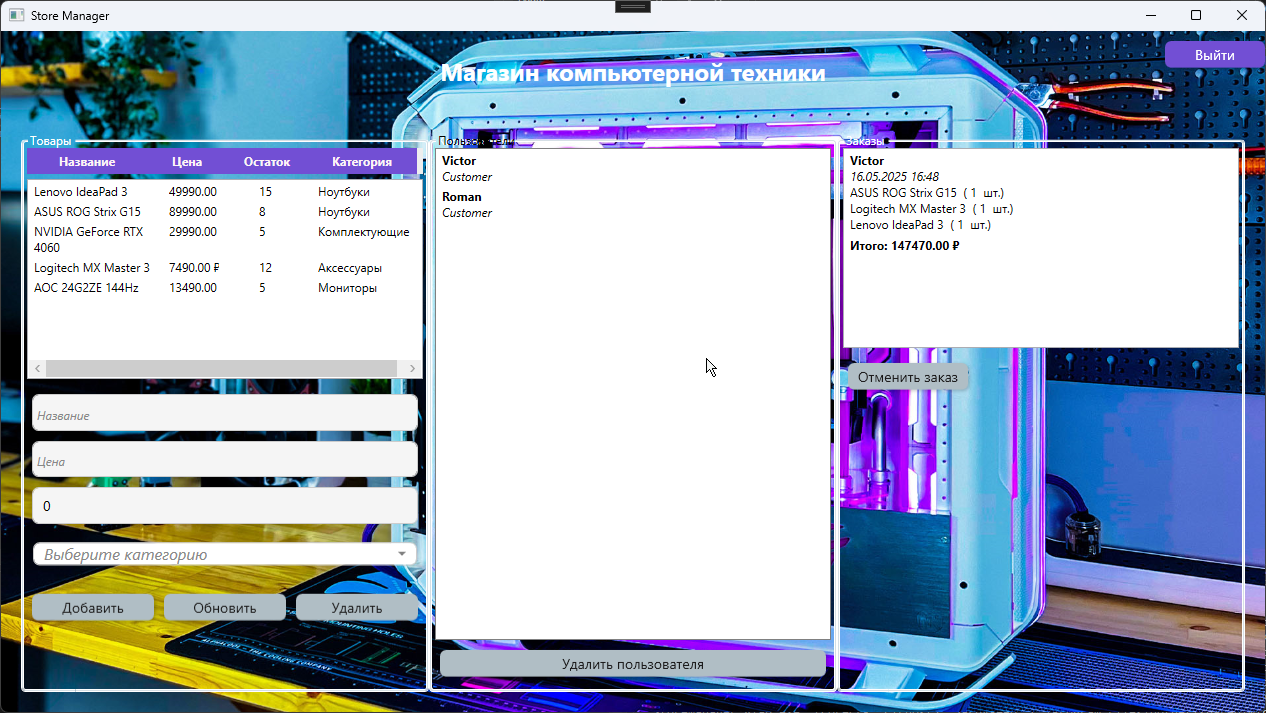
\includegraphics[width=0.8\textwidth]{fig/2025-05-18-14-37-06.png}
	\caption{Добавление товаров}
	\label{fig:add_goods}
\end{figure}

Далее необходимо войти под каждым из пользователей и сформировать заказ (Рисунок~\ref{fig:create_order1}, Рисунок~\ref{fig:create_order2}).

\begin{figure}[H]
	\centering
	
\includegraphics[width=0.8\textwidth]{fig/5.png}
	\caption{Создание заказов у первого пользователя}
	\label{fig:create_order1}
\end{figure}

\begin{figure}[H]
	\centering
	
\includegraphics[width=0.8\textwidth]{fig/6.png}
	\caption{Создание заказов у второго пользователя}
	\label{fig:create_order2}
\end{figure}

Затем, выйдя из аккаунта пользователя, необходимо войти в аккаунт администратора и по нажатию на конкретного пользователя просмотреть список его заказов.
Также у администратора есть возможность отменить конкретный заказ, созданный пользователем, а также самого пользователя и все созданные им заказы (Рисунок~\ref{fig:view_orders_admin}, Рисунок~\ref{fig:delete_user_admin}).

\begin{figure}[H]
	\centering
	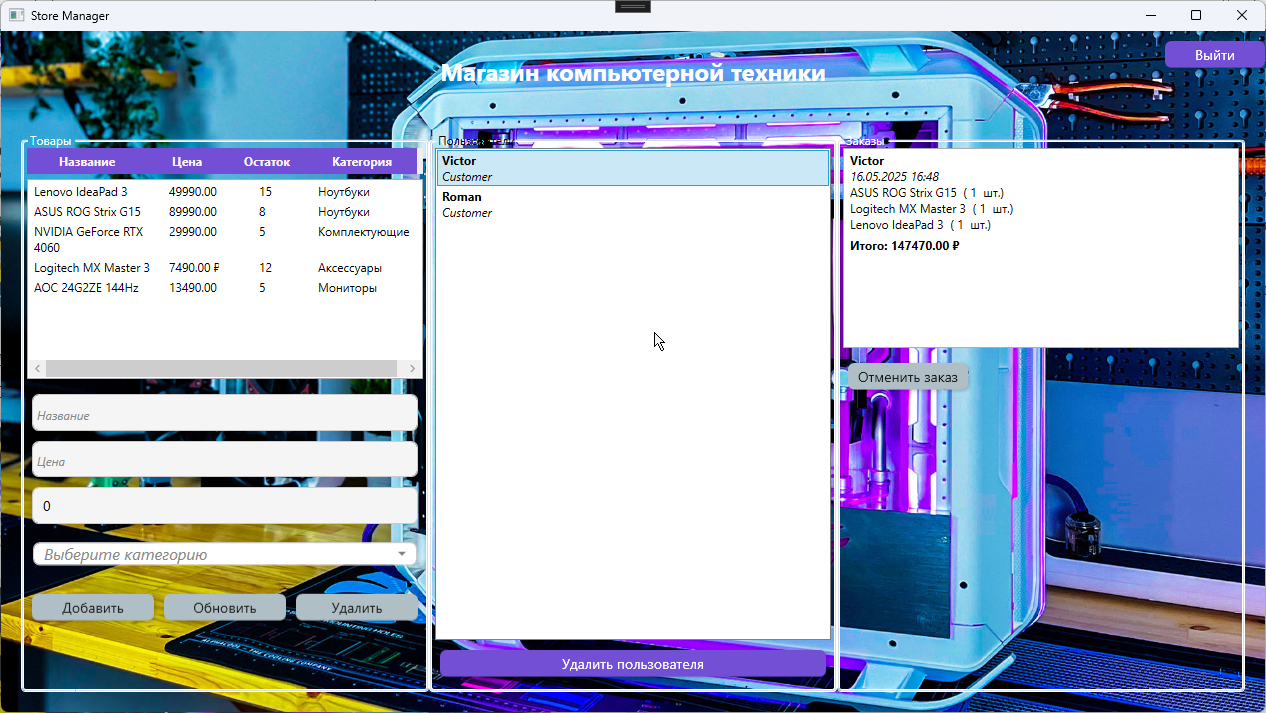
\includegraphics[width=0.8\textwidth]{fig/7.png}
	\caption{Просмотр заказов пользователя}
	\label{fig:view_orders_admin}
\end{figure}

\begin{figure}[H]
	\centering
	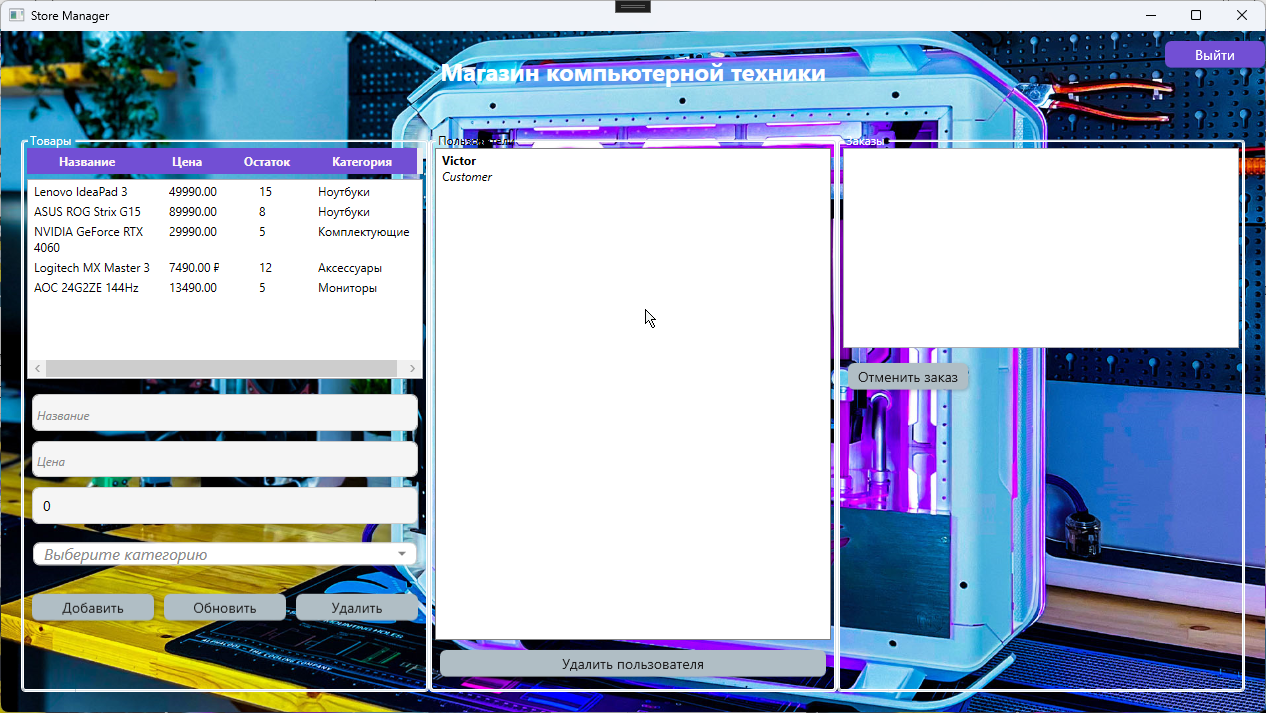
\includegraphics[width=0.8\textwidth]{fig/8.png}
	\caption{Удаление пользователя}
	\label{fig:delete_user_admin}
\end{figure}

\newpage

\section{Список вопросов}
\begin{enumerate}
	\item Как в ASP.NET Core реализуется ограничение доступа к методам только для пользователей с ролью \texttt{Admin}?
	\item Как \texttt{OrderController} определяет, какие заказы должен видеть пользователь?
	\item Как реализован вывод заказов конкретного пользователя по его \texttt{userId}?
	\item Почему при создании заказа значения \texttt{UserId} и \texttt{CustomerName} берутся из токена, а не передаются вручную?
	\item Чем отличается поведение интерфейса для администратора и для обычного пользователя?
	\item Как реализовано отображение заказов выбранного пользователя на клиенте?
	\item Как работает команда удаления пользователя на клиенте?
	\item Как настраивается каскадное удаление заказов при удалении пользователя в Entity Framework Core?
	\item Почему каскадное удаление может не сработать, даже если оно задано в \texttt{DbContext}?
	\item Как проверить, что заказы действительно удаляются при удалении пользователя?
\end{enumerate}
\end{document}
